\documentclass{article}
\usepackage[utf8]{inputenc}

\title{CSE3666 — Lab 4}
\author{Mike Medved}
\date{February 18th, 2022}

\usepackage{color}
\usepackage{amsthm}
\usepackage{amssymb} 
\usepackage{amsmath}
\usepackage[margin=1in]{geometry} 
\usepackage{listings}
\usepackage{xcolor}
\usepackage{listings}
\usepackage{graphicx}

\newcommand*\BitAnd{\mathbin{\&}}
\newcommand*\BitOr{\mathbin{|}}
\newcommand*\ShiftLeft{\ll}
\newcommand*\ShiftRight{\gg}
\newcommand*\BitNeg{\ensuremath{\mathord{\sim}}}

\lstset{frame=tb,
    language=[LaTeX]TeX,
    aboveskip=3mm,
    belowskip=3mm,
    showstringspaces=false,
    columns=flexible,
    basicstyle={\small\ttfamily},
    numbers=none,
    numberstyle=\tiny\color{gray},
    keywordstyle=\color{blue},
    commentstyle=\color{dkgreen},
    stringstyle=\color{mauve},
    breaklines=true,
    breakatwhitespace=true,
    tabsize=3
}

\lstdefinelanguage[mips]{Assembler}{%
  % so listings can detect directives and register names
  alsoletter={.\$},
  % strings, characters, and comments
  morestring=[b]",
  morestring=[b]',
  morecomment=[l]\#,
  % instructions
  morekeywords={[1]abs,abs.d,abs.s,add,add.d,add.s,addi,addiu,addu,%
    and,andi,b,bc1f,bc1t,beq,beqz,bge,bgeu,bgez,bgezal,bgt,bgtu,%
    bgtz,ble,bleu,blez,blt,bltu,bltz,bltzal,bne,bnez,break,c.eq.d,%
    c.eq.s,c.le.d,c.le.s,c.lt.d,c.lt.s,ceil.w.d,ceil.w.s,clo,clz,%
    cvt.d.s,cvt.d.w,cvt.s.d,cvt.s.w,cvt.w.d,cvt.w.s,div,div.d,div.s,%
    divu,ecall,eret,floor.w.d,floor.w.s,j,jal,jalr,jr,l.d,l.s,la,lb,lbu,%
    ld,ldc1,lh,lhu,li,ll,lui,lw,lwc1,lwl,lwr,madd,maddu,mfc0,mfc1,%
    mfc1.d,mfhi,mflo,mov.d,mov.s,move,movf,movf.d,movf.s,movn,movn.d,%
    movn.s,movt,movt.d,movt.s,movz,movz.d,movz.s,msub,msubu,mtc0,mtc1,%
    mtc1.d,mthi,mtlo,mul,mul.d,mul.s,mulo,mulou,mult,multu,mulu,mv,neg,%
    neg.d,neg.s,negu,nop,nor,not,or,ori,rem,remu,rol,ror,round.w.d,%
    round.w.s,s.d,s.s,sb,sc,sd,sdc1,seq,sge,sgeu,sgt,sgtu,sh,sle,%
    sleu,sll,sllv,slt,slti,sltiu,sltu,sne,sqrt.d,sqrt.s,sra,srav,srl,%
    srlv,sub,sub.d,sub.s,subi,subiu,subu,sw,swc1,swl,swr,syscall,teq,%
    teqi,tge,tgei,tgeiu,tgeu,tlt,tlti,tltiu,tltu,tne,tnei,trunc.w.d,%
    trunc.w.s,ulh,ulhu,ulw,ush,usw,xor,xori},
  % assembler directives
  morekeywords={[2].align,.ascii,.asciiz,.byte,.data,.double,.extern,%
    .float,.globl,.half,.kdata,.ktext,.set,.space,.text,.word},
  % register names
  morekeywords={[3]\$0,\$1,\$2,\$3,\$4,\$5,\$6,\$7,\$8,\$9,\$10,\$11,%
    \$12,\$13,\$14,\$15,\$16,\$17,\$18,\$19,\$20,\$21,\$22,\$23,\$24,%
    \$25,\$26,\$27,\$28,\$29,\$30,\$31,%
    \$zero,\$at,\$v0,\$v1,\$a0,\$a1,\$a2,\$a3,\$t0,\$t1,\$t2,\$t3,\$t4,
    \$t5,\$t6,\$t7,\$s0,\$s1,\$s2,\$s3,\$s4,\$s5,\$s6,\$s7,\$t8,\$t9,%
    \$k0,\$k1,\$gp,\$sp,\$fp,\$ra},
}[strings,comments,keywords]

\definecolor{CommentGreen}{rgb}{0,.6,0}
\lstset{
  language=[mips]Assembler,
  escapechar=@, % include LaTeX code between `@' characters
  keepspaces,   % needed to preserve spacing with lstinline
  basicstyle=\small\ttfamily\bfseries,
  commentstyle=\color{CommentGreen},
  stringstyle=\color{cyan},
  showstringspaces=false,
  keywordstyle=[1]\color{blue},    % instructions
  keywordstyle=[2]\color{magenta}, % directives
  keywordstyle=[3]\color{red},     % registers
}

\begin{document}
\graphicspath{ {.} }

\maketitle

\section{Prompt}
In this lab, we refactor the code we wrote in lab 3. We will implement two functions.

\begin{enumerate}
    \item \textbf{Remove Spaces}
    $\hfill \break$
    This is a leaf function. We can copy the code in Step 2 from lab3. Revise it if necessary. Note the following:
        \begin{itemize}
            \item  str and res are strings. Like an array, when we pass a string to a function, we only put its starting address in an argument register. For example, register a0 has the starting address of string str.
            \item  This function is a leaf function. It does not need to use the stack.
            \item  The function does not return a value.
        \end{itemize}
    \item \textbf{Print Non-Spaces}
    $\hfill \break$
    The second function is print\_ns. The prototype is as follows.
    The steps to be implemented in the function are listed below. Do NOT use la. All the information the function needs is the argument.
    \begin{itemize}
        \item Save registers. This step should be done later after Steps 2 to 4 are completed.
        \item Create local array res of 128 bytes on the stack. We only need to move the stack pointer to allocate space (128 bytes) for the string.
        \item Call remove\_spaces function to remove spaces in s and save the result in res. $\hfill \break$ Note that we need to put string s's address in a0, and res's address in a1.
        \item Print res with a system call.
        \item Restore registers and stack, and return s.
    \end{itemize}
    Clearly mark each step in your code. Again, we write code for Steps 2, 3, and 4 first so that we know what registers to save and restore in Steps 1 and 5.
    $\hfill \break$

    Step through the function and observe the values in registers ra and sp.
    $\hfill \break$
    Also examine the stack in Data Segment window.

\end{enumerate}

\break
\section{Deliverables}
    \begin{lstlisting}
    print_ns:
        # store the result pointer in a1
        add  a1, sp, x0

        # allocate 136 bytes to the stack
        # - 128 for the string
        # - 4 for the return address
        # - 4 for the original string
        addi  sp, sp, -136

        sw    ra, 4(sp)      # store current return address on the stack
        sw    a0, 0(sp)      # preserve original string so we can return it later
        jal   remove_spaces  # invoke remove_spaces

        # use system call 4 to print the result to stdout
        addi  a0, a1, 0
        addi  a7, x0, 4
        ecall

        # restore state so we can return back to the main loop
        lw    ra, 4(sp)
        lw    a0, 0(sp)
        addi  sp, sp, 136
        jr    ra
    \end{lstlisting}

\section{Run Examples}
\begin{lstlisting}[language=Java]
a b c
abc

abcd e
abcdef

ab c d e f gh i j
abcdefghij

abcdefghijklmnopqrstuvwxyz
abcdefghijklmnopqrstuvwxyz

This string has escape sequences \n and special characters **
Thisstringhasescapesequences\nandspecialcharacters**

RISC-V: The Free and Open RISC Instruction Set Architecture
RISC-V:TheFreeandOpenRISCInstructionSetArchitecture

This string has lots of spaces and other funny characters!!!
Thisstringhaslotsofspacesandotherfunnycharacters!!!
\end{lstlisting}

\section{Data Segment View}
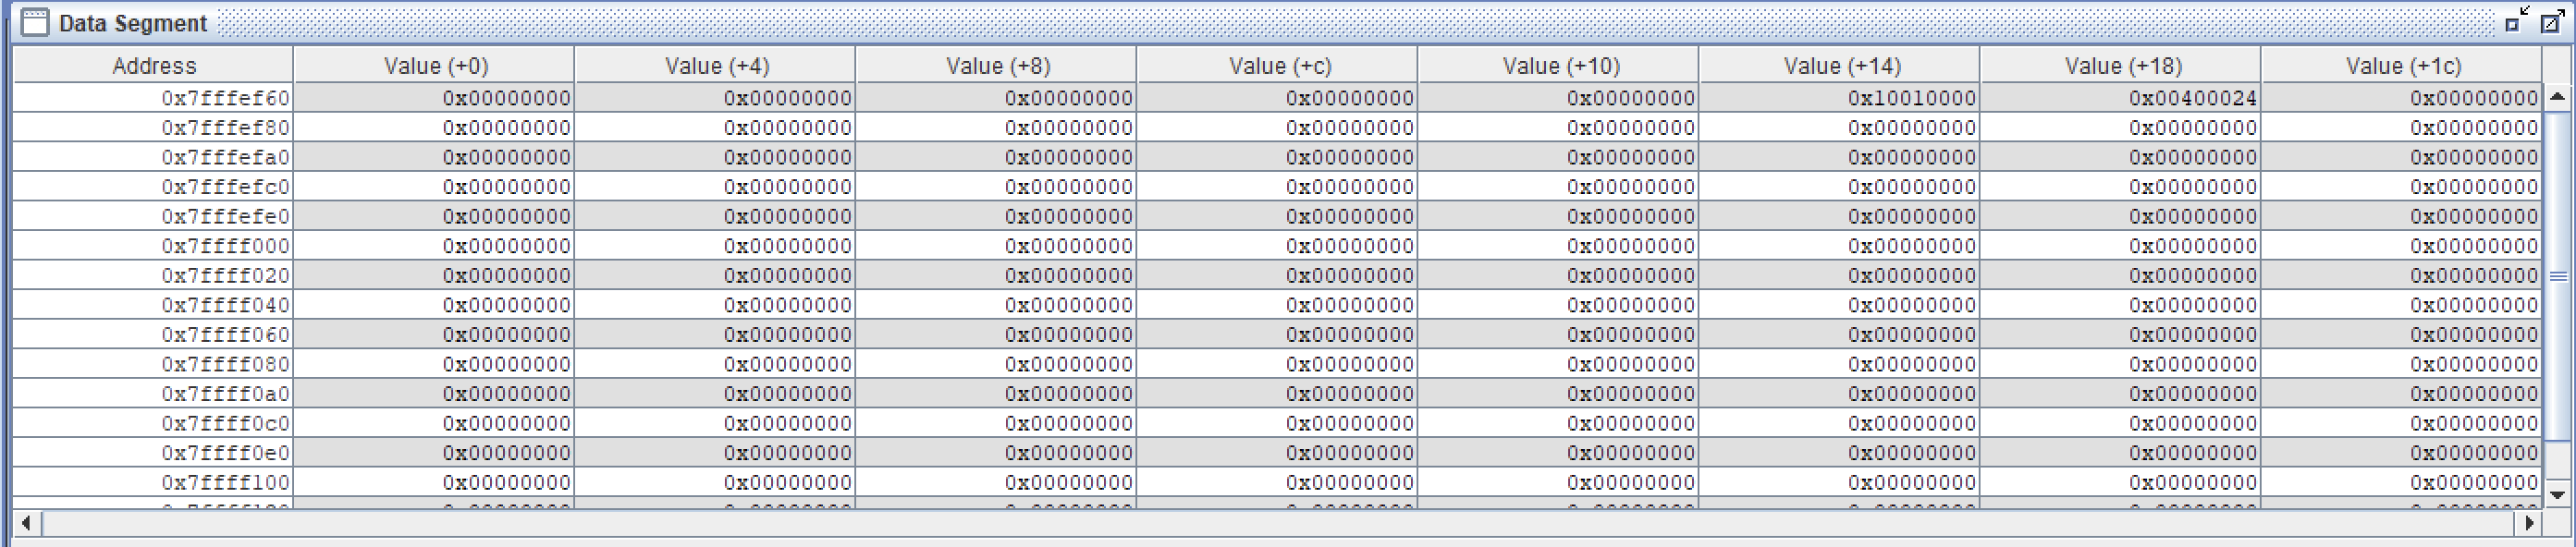
\includegraphics[width=15cm]{addr}

\end{document}
